% !TEX root =  main.tex

\chapter{Design}
The platform will consist of one main server application with an attached database. 

It is intended to be deployed on a Beckhoff CX2030 PC. This machine has a dual-core Intel Core i7 1.5GHz CPU and up to 4GB RAM. The disk is a flash card. The machine is intended to reside in the same building as the devices it should interact with.

\section{Database design}
Since the intended machine is somewhat limited, the immediate choice would be to use SQLite for the database.
SQLite is however not designed for concurrent access, in that it resides in a single file which must be locked to perform writes. Supporting 5-600 writes per second (the Grundfoss dormitory) from multiple data provider threads/processes along with controller processes, monitor processes, a reporting process and a predictor process is expected to cause significant file lock contention. \textgreater500 writes per second gives \textless2ms per write, not counting the need to allow other processes to access the database. Since we do not expect to do disk writes in less than 2ms (and even if we did, there would be no scaling potential), the SQLite option is abandoned.

The database will reside in a PostgreSQL DBMS which is open source and should run well even on a smaller machine.

\subsection{Schema: core}
The central part of the database schema is shown in figure \ref{figureDbCoreModel} and explained below:

\begin{figure}[H]
    \centering
    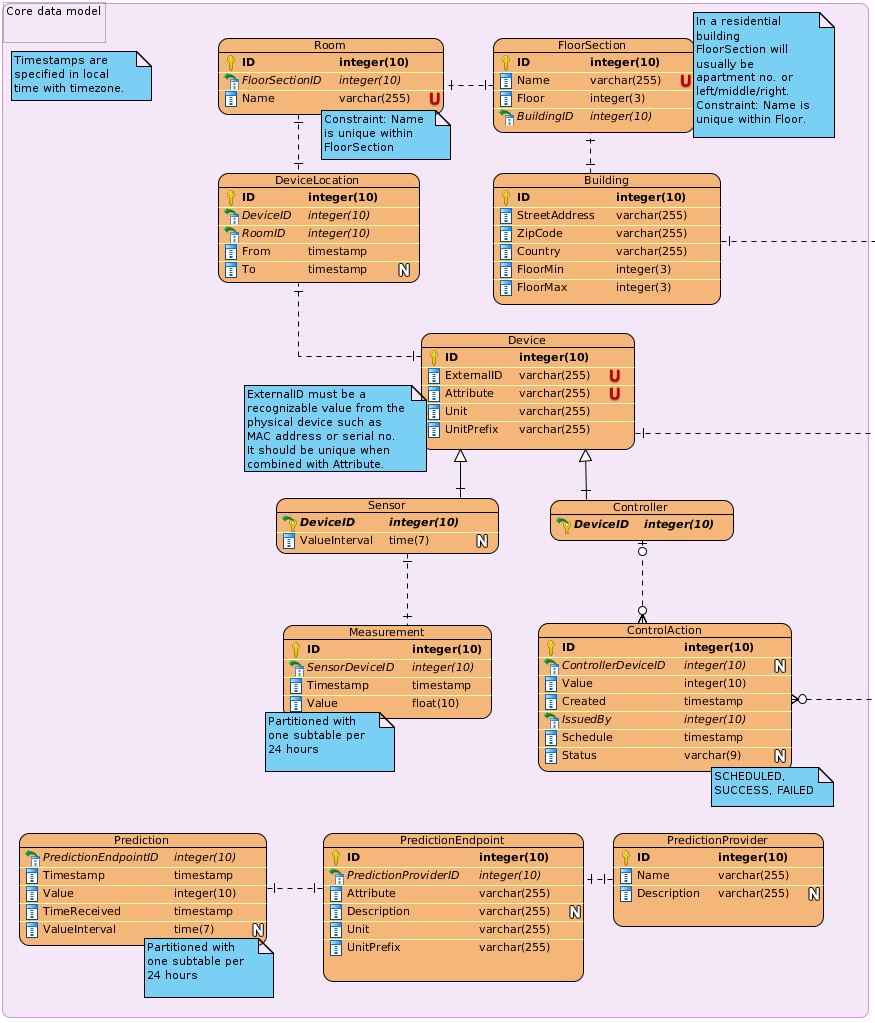
\includegraphics[width=\textwidth]{figures/db_core_schema}
    \caption{Database core schema}
    \label{figureDbCoreModel}
\end{figure}

\subsubsection{Devices and measurements}

\paragraph{Device} 
Entries in \texttt{Device} correspond to physical control and sensor devices, with the modification that we store one logical device for each function of the physical device. Whether a device is a sensor or a controller is specified by its presence in table \texttt{Controller} or \texttt{Sensor}. Columns \texttt{Attribute}, \texttt{Unit} and \texttt{UnitPrefix} (such as milli) are for sensors specification of the incoming measurement values, while they for controllers specify the format of values to send to the controller when actuating it.

\paragraph{Sensor} 
Table \texttt{Sensor} specifies an optional property \texttt{ValueInterval} which is used when measurement values are aggregated over a limited time interval (such as 15 minutes). 

\paragraph{Measurement} 
This table will contain a row for each measurement received from a physical sensor. It will simply consist of a \texttt{Value}, a \texttt{Timestamp} and a reference into \texttt{Sensor}, which enables interpretation of the value. The \texttt{Measurement} table is expected to grow very large and will therefore be partitioned into subtables that will each contain 24 hours of measurements and can be discarded on the fly according to the rolling window strategy explained in section \ref{subsection:rollingwindow}.

\paragraph{ControlAction} 
Table \texttt{ControlAction} will contain scheduled and past commands for controllers. An action is simply specified by a \texttt{Value} which can be interpreted via the reference into table \texttt{Controller} and \texttt{Device}. Column \texttt{Schedule} specifies the time for carrying out the action, and \texttt{Status} indicates if execution is still pending or has been completed. Finally, \texttt{IssuedBy} specifies which user scheduled the action. We might consider partitioning and discarding of old data in this table in the same way as for table \texttt{Measurement}.

\paragraph{Building, FloorSection, Room}
The physical properties of a building are modeled in these tables. A building consists of an integer range of floors. Each floor consists of \texttt{FloorSection}s which in most cases will be equivalent to apartments. The generalized term FloorSection is intended to support other types of buildings where designations such as "South wing" or other may be desired. Finally, a floor consists of named \texttt{Room}s. We do not expect to obtain device locations with a higher degree of accuracy than individual rooms.

\paragraph{DeviceLocation} This table maps \texttt{Device}s to \texttt{Room}s for specified time periods, indicating that devices may be moved around.

\subsubsection{Predictions}
Predictions of a wide range of values (power consumption, grid load, price, CO\textsubscript{2} emissions, ...) will be received from external data providers and will in addition be generated by our own application logic. 

While the data stored for predictions is quite similar to those for measurements, we have chosen to store them separately because of the fundamentally different semantics.

\paragraph{PredictionProvider}
An entity providing predictions, such as energinet.dk or the system itself.

\paragraph{PredictionEndpoint} 
A logical source of predictions of one type. Specifies the \texttt{Attribute}, \texttt{Unit} and \texttt{UnitPrefix} of the incoming values and provides an optional \texttt{Description}.

\paragraph{Prediction}
Actual prediction values. \texttt{Timestamp} indicates the time for which the value applies, while \texttt{TimeReceived} indicates when the prediction was received from the provider. This is relevant since multiple predictions for the same future point in time may be received over time. Some values actually cover an interval (for instance predicted power consumption for a given day of 24 hours), which is specified in column \texttt{ValueInterval}.
This table is also expected to grow quickly, motivating the same partitioning and rolling window strategy as for table \texttt{Measurement}.

\newpage
\subsection{Schema: Users, groupings and privileges}

The database schema for storing device groupings, users, user groups and their privileges has been developed to meet the requirements from section \ref{subsection:PrivilegesRequirements}. This is shown below:

\begin{figure}[H]
    \centering
    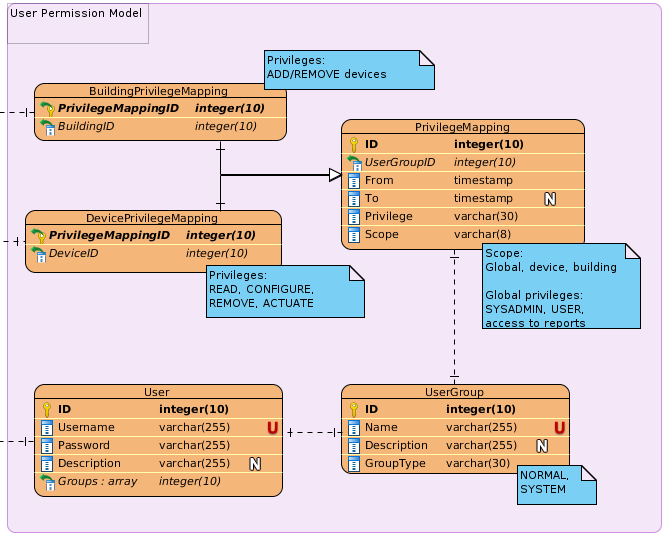
\includegraphics[width=\textwidth]{figures/db_user_schema}
    \caption{Schema for device groups, user groups and privileges}
\end{figure}

\paragraph{DeviceGroupMapping}
Devices can be put in arbitrary logical groups which is modeled by this table.

\paragraph{User and UserGroup}
\texttt{User}s have a username and a password (which will be hashed with a suitable one-way hash function) and can be member of a number of \texttt{UserGroup}s.

\paragraph{HierarchyGroup and HierarchyMapping} 
\texttt{DeviceGroup} and \texttt{UserGroup} are subtypes of the general \texttt{HierarchyGroup} which can be nested in parent-child relationships as modeled by \texttt{HierarchyMapping}.

\paragraph{PrivilegeMapping}
This table maps \texttt{UserGroup}s to specific privileges. A mapping includes a time period which may be open-ended. In order to have privileges for specific devices and buildings as well as globally valid ones, a \texttt{Scope} must be set. In case of a device or building-specific privilege, the concerned \texttt{DeviceGroup} or \texttt{Building} must be looked up in \texttt{DevicePrivilegeMapping} or \texttt{BuildingPrivilegeMapping} respectively. These tables are intended to have corresponding subtypes in the object-oriented implementation.

It will be up to application logic to interpret the semantics of the concrete privileges.



\subsection{Subject to change}
We can already foresee that configuration of controllers as well as other settings that must be persisted will most likely require extensions to the schema proposed above. The basic structure of the core schema should however not change.

\subsection{Rolling window}\label{subsection:rollingwindow}
Since the \texttt{Measurement} table will grow very quickly, a partitioning and data discarding scheme will be employed. The table will be partitioned in time intervald, having one subtable for every 24 hours. Furthermore, subtables older than one week will be dropped. The time limits can naturally be configured. The same scheme might be applied to tables \texttt{ControlAction} and \texttt{Prediction}.
This is done in order to accommodate the VPP server on a desktop size machine with limited disk space.

\subsection{Data warehouse}
In order to retain data, the VPP will periodically forward data to an external database (data warehouse) that can accommodate a larger volume of data for longer periods. When forwarding data, measurements may be averaged over limited time intervals to reduce data size. The data warehouse can then be used for statistics and historical analysis. While the data warehouse schema was initially planned to be identical to the VPP rolling window DB, the presence of users, privileges and most likely various other configuration indicates that probably only the core schema as shown in figure \ref{figureDbCoreModel} should be present in the data warehouse. 

\subsection{CIM compliance}
The Common Information Model (CIM) is being taken into consideration in the design. Where it is applicable, we will aim to make our data model compliant. Units, unit prefixes, timestamps and time durations will be formatted to agree with CIM. On the other hand, CIM does not provide any guidance on how to structure for instance the building/floor/room model.

\newpage
\section{Application design}
The application will be programmed in object-oriented Python, using Python processes to enable concurrent processing. 

Using processes instead of threads is necessary to utilize both cores in the intended machine, since Python employs a \emph{Global Interpreter Lock} which prevents threads within the same Python interpreter from executing concurrently. Using processes mitigates this as each process will run with its own interpreter. 

\subsection{Static structure}
structure is shown in figure \ref{figureClassDiagram} and elaborated below:

\begin{figure}[H]
    \centering
    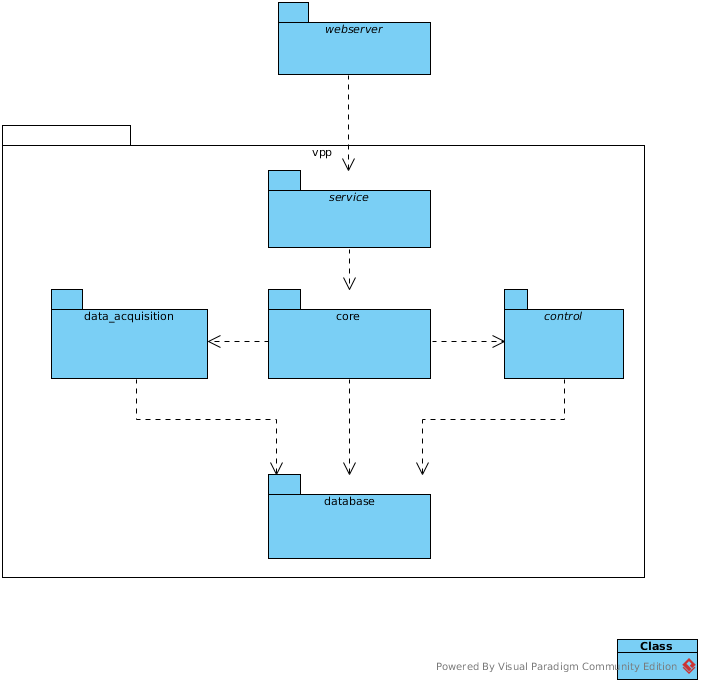
\includegraphics[width=\textwidth]{figures/class_overview}
    \caption{Class diagram. }
    \label{figureClassDiagram}
\end{figure}

The server application is roughly structured in a three-layered architecture with the \texttt{database} at lowest layer, the \texttt{core}, \texttt{control} and \texttt{data\_acquisition} packages as the middle "domain" layer and the \texttt{service} package as the top layer, providing an external interface. 

The \texttt{webserver} will access the \texttt{service} layer to provide GUI. It will be a separate application deployed on the same machine. See section \ref{subsection:webserver}.



\subsubsection{Package \texttt{vpp.core}}
This package implements the core logic of the VPP server. Classes are explained in detail below.

\begin{figure}[H]
    \centering
    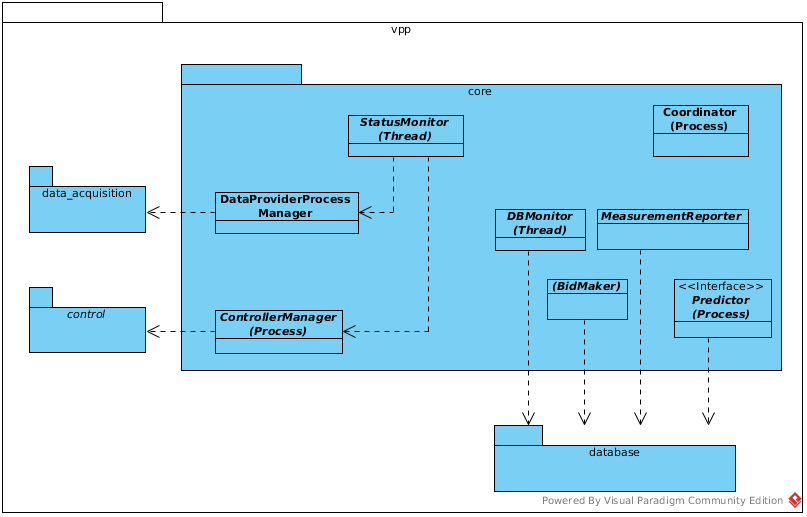
\includegraphics[width=\textwidth]{figures/class_core}
    \caption{Core}
    \label{figureClassDiagram}
\end{figure}

\texttt{Coordinator} is responsible for instantiating other classes and processes. For clarity, associations are not shown in the diagram.\\

\texttt{DataProviderProcessManager} launches the process which instantiates and manages the individual data providers that will supply measurements and predictions. \\

\texttt{ControllerManager} instantiates and keeps track of controllers for actuating physical devices. This will run in a separate process that periodically will check for and execute scheduled actions. It is expected that one process for handling all actions will be sufficient. \\

\texttt{StatusMonitor} runs a process that will poll \texttt{DataProviderManager} and \texttt{ControllerManager} for status and make this information available to the service layer.\\

\texttt{DBMonitor} runs a process that will monitor the database status. It will give information on when the last measurements were received and similar.\\

\texttt{Predictor} will run a process to create predictions based the available data.\\

\texttt{DBAccess} provides a clean interface for retrieving and posting data from and to the database. 

\subsubsection{Package \texttt{vpp.data\_acquisition}}

\begin{figure}[H]
    \centering
    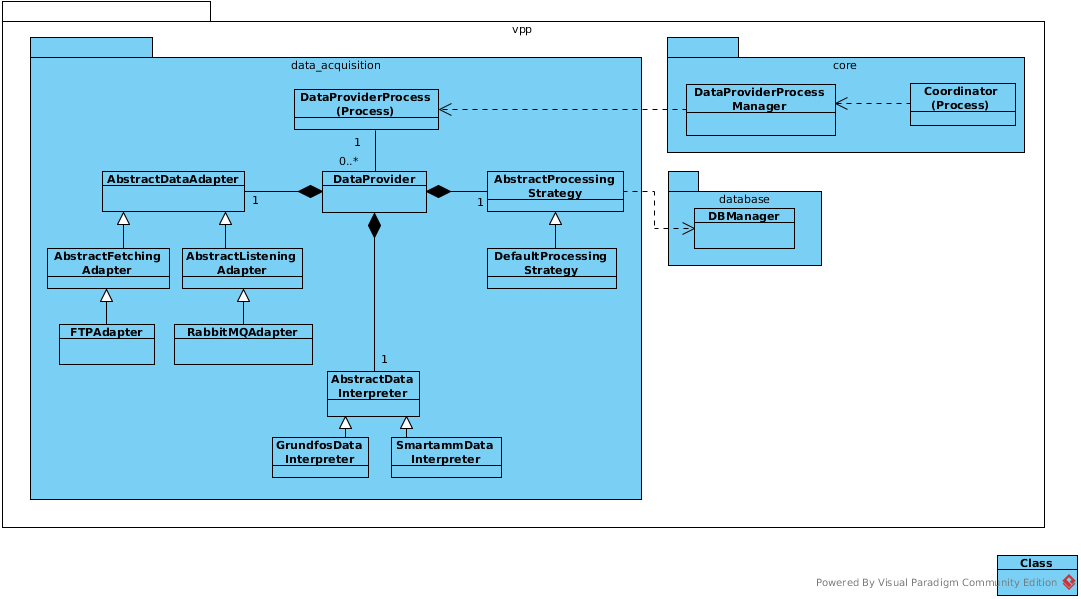
\includegraphics[width=\textwidth]{figures/class_data_acquisition}
    \caption{Data acquisition}
    \label{figureClassDiagram}
\end{figure}

This package contains the framework for connecting to various sources of measurement and prediction data. Class \texttt{DataProvider} can be instantiated in a separate thread to model a single source of data. Each \texttt{DataProvider} instance employs a suitable \texttt{DataAdapter} to communicate with for instance a message queue or a SmartAmm server.

A distinction is made between listening adapters (\texttt{AbstractListeningAdapter}), which will be activated by external events, and fetching adapters (\texttt{AbstractFetchingAdapter}) which employ an internal timer to fetch data periodically.

\subsubsection{Package \texttt{vpp.control}}
Similar to \texttt{data\_acquisition}, this package will provide a framework for communicating with the various control devices. A \texttt{Controller} can be instantiated with a suitable \texttt{ControllerAdapter} to communicate with a given device. 


\subsubsection{Package \texttt{vpp.database}}
This package contains the code that interfaces directly with the database. 

\texttt{DBMaintainer} will run maintenance on the database and implement the Rolling Window strategy.

Communication with the database could be implemented simply using SQL, or we could opt for an object-relational mapper (ORM) framework such as SQLAlchemy.


\subsection{Runtime processes}

The runtime creation of processes within the main server application is shown below:
\begin{figure}[H]
    \centering
    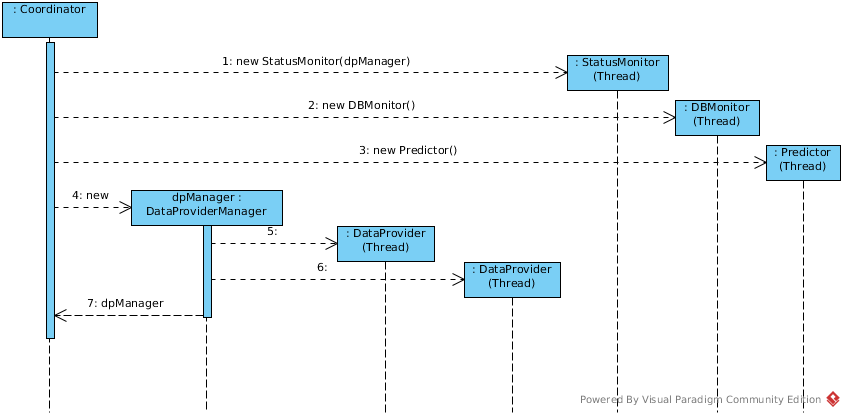
\includegraphics[width=\textwidth]{figures/seq_diagram}
    \caption{Sequence diagram of thread creation}
    \label{figureSeqDiagram}
\end{figure}
As can be seen, at least six concurrent processes will be running in addition to any \texttt{DataProviders} configured.


\subsubsection{Process communication overhead}
There is of course an overhead cost involved in running processes as opposed to threads, since processes do not have shared memory which will make communication more costly performance-wise. A balanced approach could be to group processes with frequent communication as threads within the same process, thus reducing the total number of processes form the current minimum six (plus \texttt{DataProviders}) to two or three. 

\newpage
\subsection{Data acquisition}
The execution flow when receiving measurements from a RabbitMQ is shown below:
\begin{figure}[H]
    \centering
    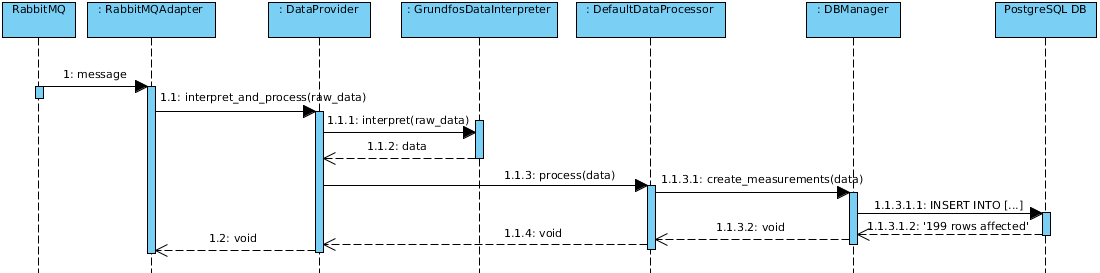
\includegraphics[width=\textwidth]{figures/data_acq_seq_diagram}
    \caption{Sequence diagram of data acquisition}
    \label{figureSeqDiagram}
\end{figure}


\subsection{Web server}\label{subsection:webserver}
We intend to provide a web interface for users to access the system. This will run in a separate web server, but in the same machine. The preliminary plan is to build the webapp using Django since this supports Python. 

The web interface could in itself grow to a rather large application with support for building configuration, device configuration, user administration, actuation interfaces and so on. This will require a substantial design and development effort. In the initial version, we plan to support only very basic interaction as proof of concept.